\chapter{Adaption of example applications}
\label{ch:adaption}
In this chapter, to show the feasibility of the approach, two open-source e-mail clients adapted to support run-time state migration based on the developed approach as part of the thesis.

As a developer who wants to implement the enabling run-time state migration, we used the developed approach, middleware, libraries, deriving interfaces, and adaptability to existing same-purpose applications. 

\section{Application State Models}
After analyzing states of these applications and their source code (Table \ref{tab:states_of_email_applications}), we decided to model \textit{search} and \textit{sending-email} states. We developed two common Application State Models for these two applications (Listing \ref{lis:search-schema} and \ref{lis:sending-email-schema}). 



\section{Example Applications}
These applications are for different platforms, and their source code is freely accessible to allow the integration of libraries. 
Suggestions for e-mail clients to be adapted are K-9 Mail for Android and Mailspring for desktop operating systems. They are interactive applications for end-users and have sufficient complexity (e.g., applications do not have only one single state).
K9-Mail Android application is developed in Java; therefore, it requires the Android library. Moreover, Mailspring is developed using Electron and Node.js for desktop operating systems, and it needs the JavaScript library.

\subsection{Mailspring}
Mailspring is an open-source e-mail client application\footnote{\url{https://getmailspring.com/}}. The source code of this application is available on GitHub\footnote{\url{https://github.com/Foundry376/Mailspring}}. This application can be installed on desktop operating systems like macOS, Linux, and Windows.
\subsubsection{Architecture}
As Mailspring is written in TypeScript and is based on Electron, the process that runs package.json's main script is called the main process. The main process's script can display a UI by generating web pages. An Electron app has only one main process. Also, Electron has another type of process, which is the renderer process, and each web page runs in its own renderer process. Electron provides a special API for communication of main process and renderer processes \cite{electron}. Furthermore, Mailspring's UI is developed in ReactJS, which is a JavaScript UI library. Each part of the UI is a ReactJS component.

\subsubsection{Adaptions}
The run-time state migration JavaScript library and Application State Models interfaces are integrated into the main process's script. On the other hand, all UI adaptions are in ReactJS components. 

Adaptions are added to the fork of this project, hosted on GitHub\footnote{\url{https://github.com/asml-lang/mailspring}}. 

\subsection{K-9 Mail}
K-9 Mail is an open-source e-mail client application\footnote{\url{https://k9mail.app/}}. The source code of this application is available on GitHub\footnote{\url{https://github.com/k9mail/k-9}}. This application can be installed on Android devices.

\subsubsection{Architecture}
K-9 Mail written in Java 8. However, the new code base is migrating to Kotlin. The K-9 Mail project consist of different modules. The \textit{k9mail} which is the main module which includes code for database interaction, notification and activities. Another module is the \textit{k9mail-library} which is the back-end code for decoding emails and contacting mail providers. 

\subsubsection{Adaptions}
As we worked only only on the application, all adaptions are implemented in \textit{k9mail} module. The run-time state migration Android library has been added to this module as a dependency. The \textit{k9mail} consist of different packages. The integration of run-time state migration is implemented in \textit{ui} package.

Adaptions are added to the fork of this project, hosted on GitHub\footnote{\url{https://github.com/asml-lang/k-9}}. 


\subsection{UI Adaptions}
In this section, we explain all implemented UI adaptions in both applications to achieve a proper behavior of run-time state migration. 

\subsubsection{Notifications}
When a device joins or leaves, other devices which are subscribe to the same Application State Model's topic will be notified by \textit{onDeviceJoin} and \textit{onDeviceLeave} callbacks. Devices who gets this message show a native notification on their application and inform the user about connectivity status of the device.

\subsubsection{Run-time State Migration Button}
For each view of a state, we developed a floating action button as the main button of run-time state migration. When the user click on this button, applications displays two other buttons as \textit{Set State} for push method and \textit{Get State} for the pull method. The user can start the migration process by clicking one of this button on the current run-time state.

\subsubsection{Device List Modal}
When the user clicks on run-time state migration button and clicks on one of migration methods' buttons, applications shows a modal window. This modal window displays the name of the current run-time state, migration method and the list of the devices that are available for migration by \textit{getDevices}. The user should select a device from the list and click on the \textit{migrate} button. By clicking on the \textit{migrate} button, If the chosen method is push, the run-time state can be migrated by \textit{sendState}. Otherwise, for the pull method, the run-time state can be requested by \textit{getStateDevice}. At the end the modal window get closed. 

\subsubsection{Run-time State Adjustments}
We adjust both applications for both \textit{search} and \textit{sending-email} states. If the target device gets a new run-time state by \textit{onStateReceive}, application react responsively. For \textit{search} state, the input of the query text gets updated with the source application's query text. Also, if the search is already submitted on the source application, the target device also tries to submit the query text and shows a result. Moreover, for \textit{sending-email} state, if the target device gets a new run-time state by push method, it displays the new draft on a new compose window. Also, user can click on the run-time state migration button on the compose window and pull and push the run-time state of the current window. After adjustment, the target device announce the end of migration with \textit{setMigration} to the source device.

\subsubsection{Removing Run-time State}
When a device gets \textit{onStateMigration}, application resets all input of the corresponding run-time state. For \textit{search} state, in query text input will be empty and the list of result will be reset. For \textit{sending-email}, the current compose window will be closed.

\subsubsection{UI Screenshots}
In this section we demonstrate UI adjustments in example applications.

Figure \ref{fig:adapt-noti} shows a run-time state migration button which belongs to \textit{search} state. Also, this figure displays notifications for joining K-9 Mail and Mailspring by sharing the \textit{search} state.


\FloatBarrier
\begin{figure}[H]
    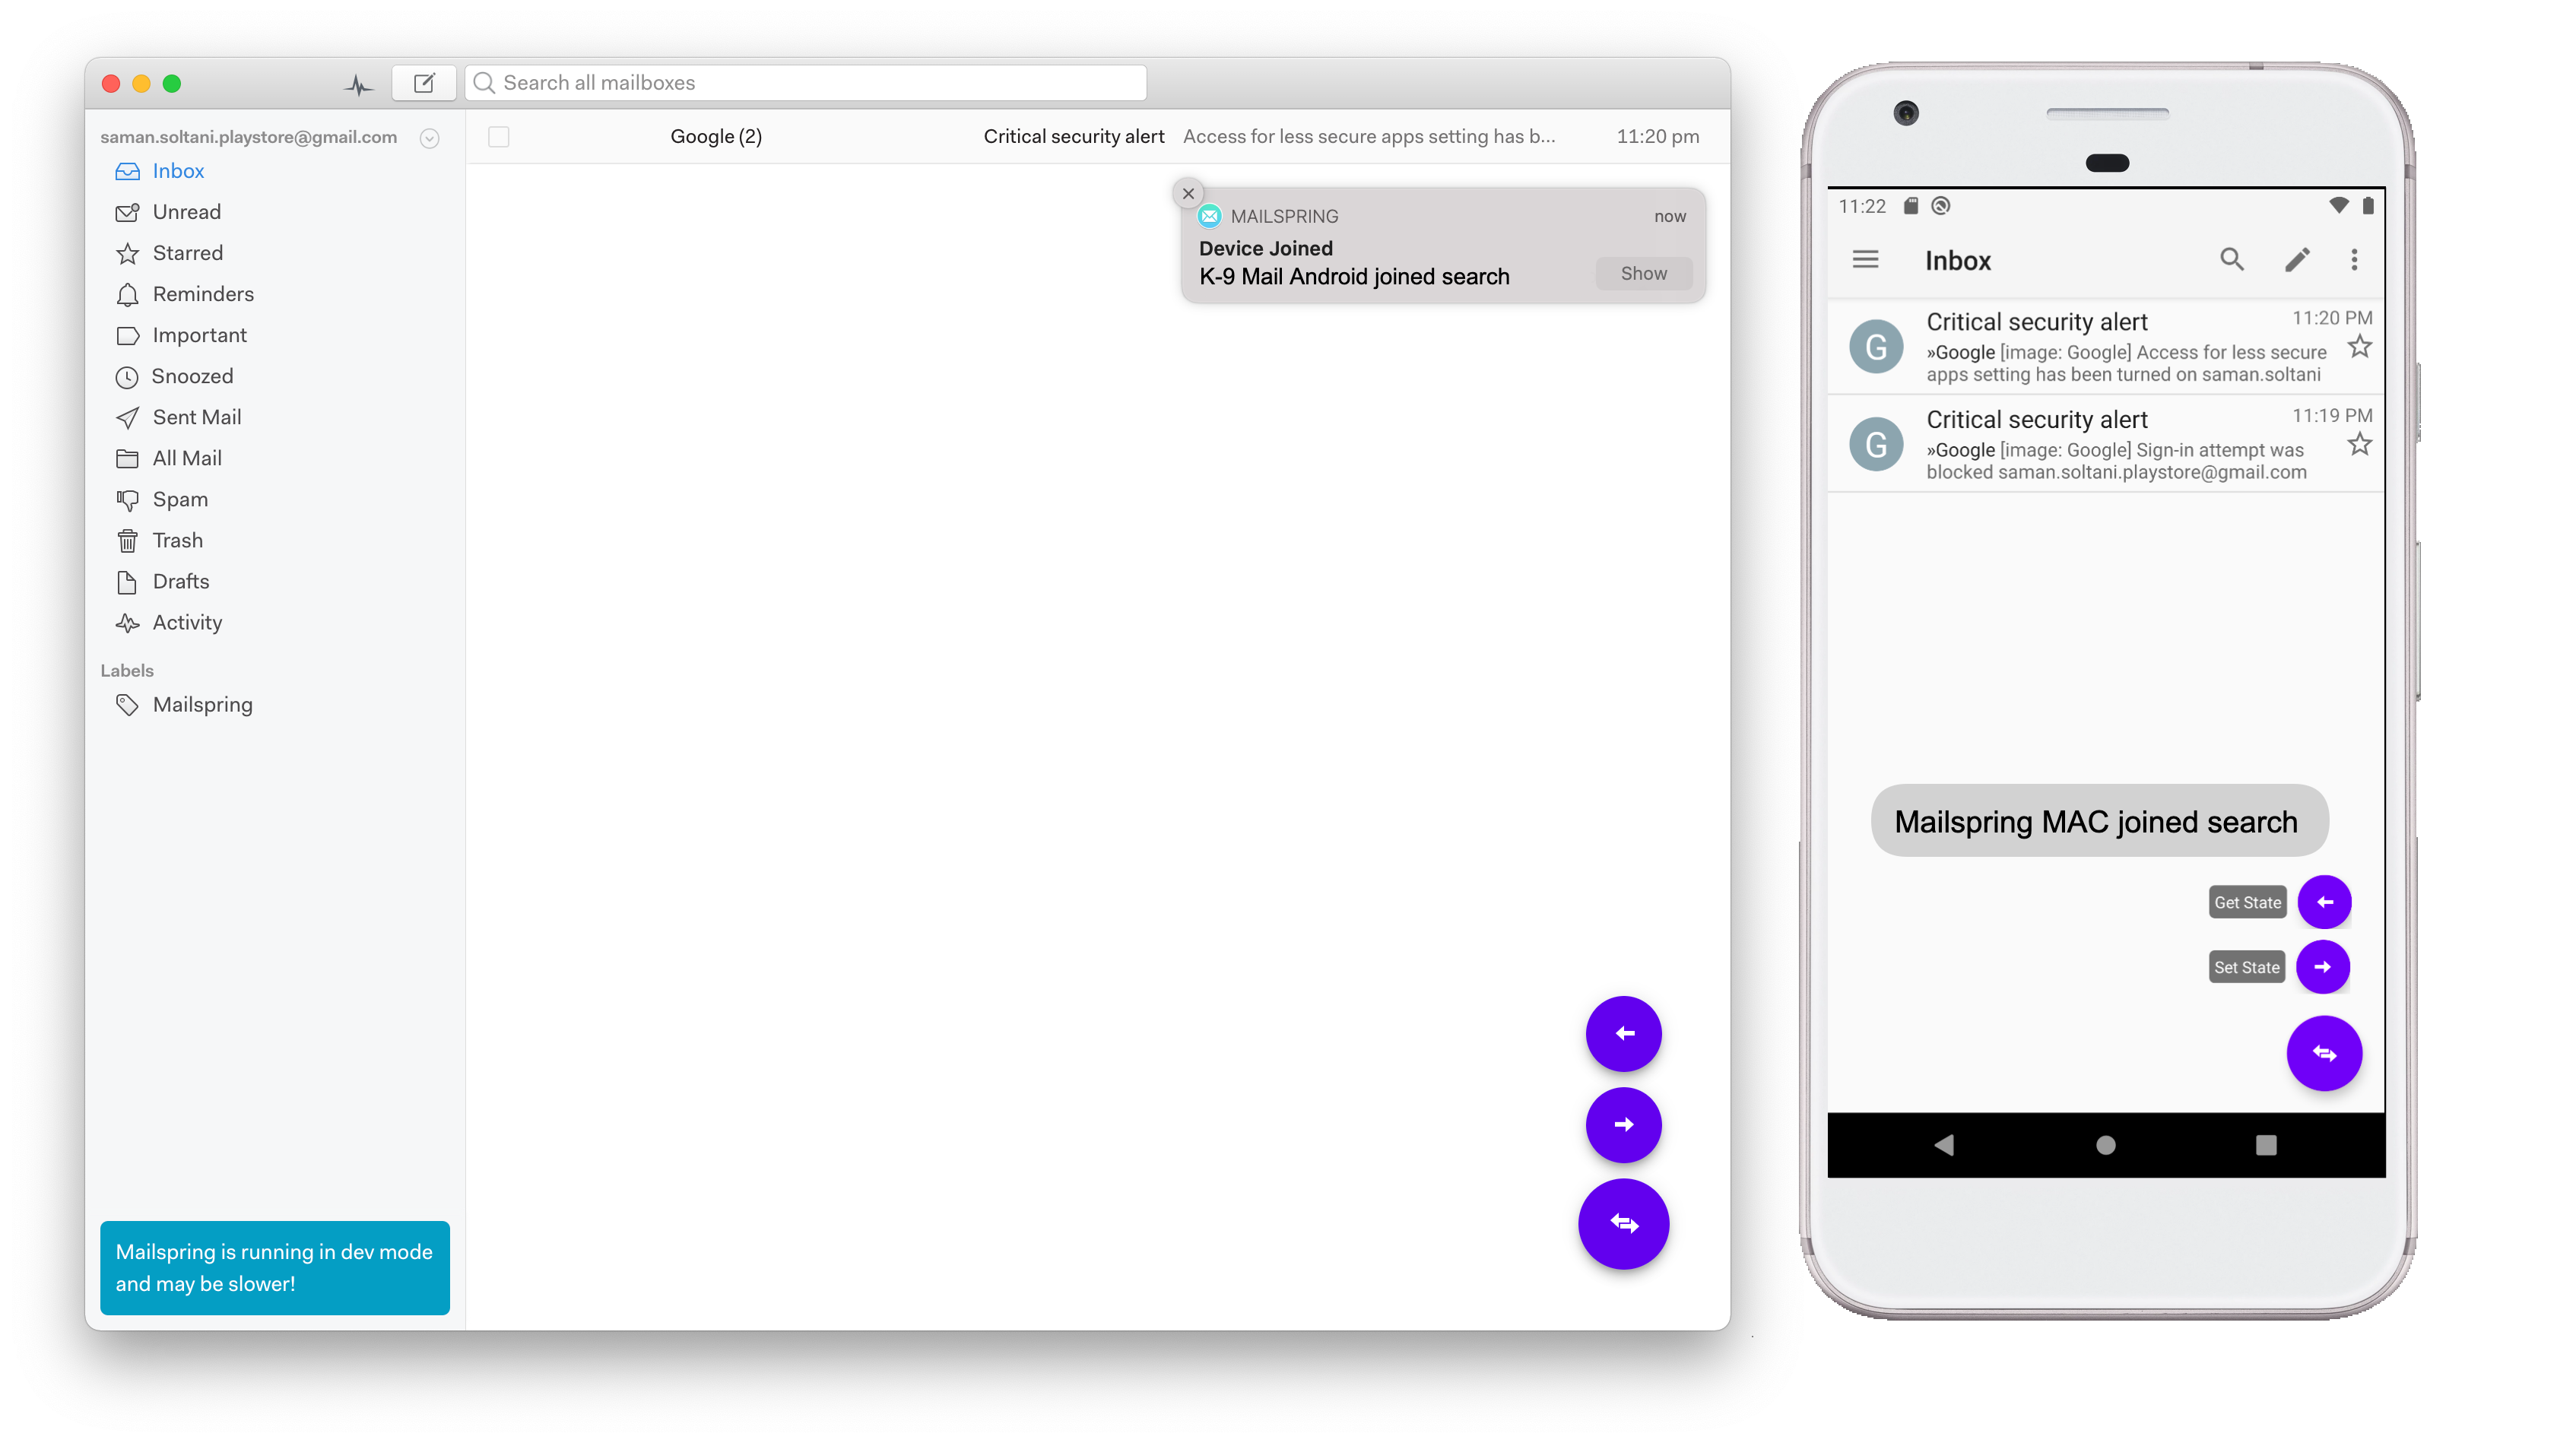
\includegraphics[width=\linewidth]{../figures/adapt-noti.png}
    \centering
    \caption{Screenshot of Native Notifications and Run-time State Migration Button}
    \label{fig:adapt-noti}
\end{figure}
\FloatBarrier

Figure \ref{fig:adapt-compose} shows the compose window of Mailspring and K-9 Mail which they have a run-time state migration button.

\FloatBarrier
\begin{figure}[H]
    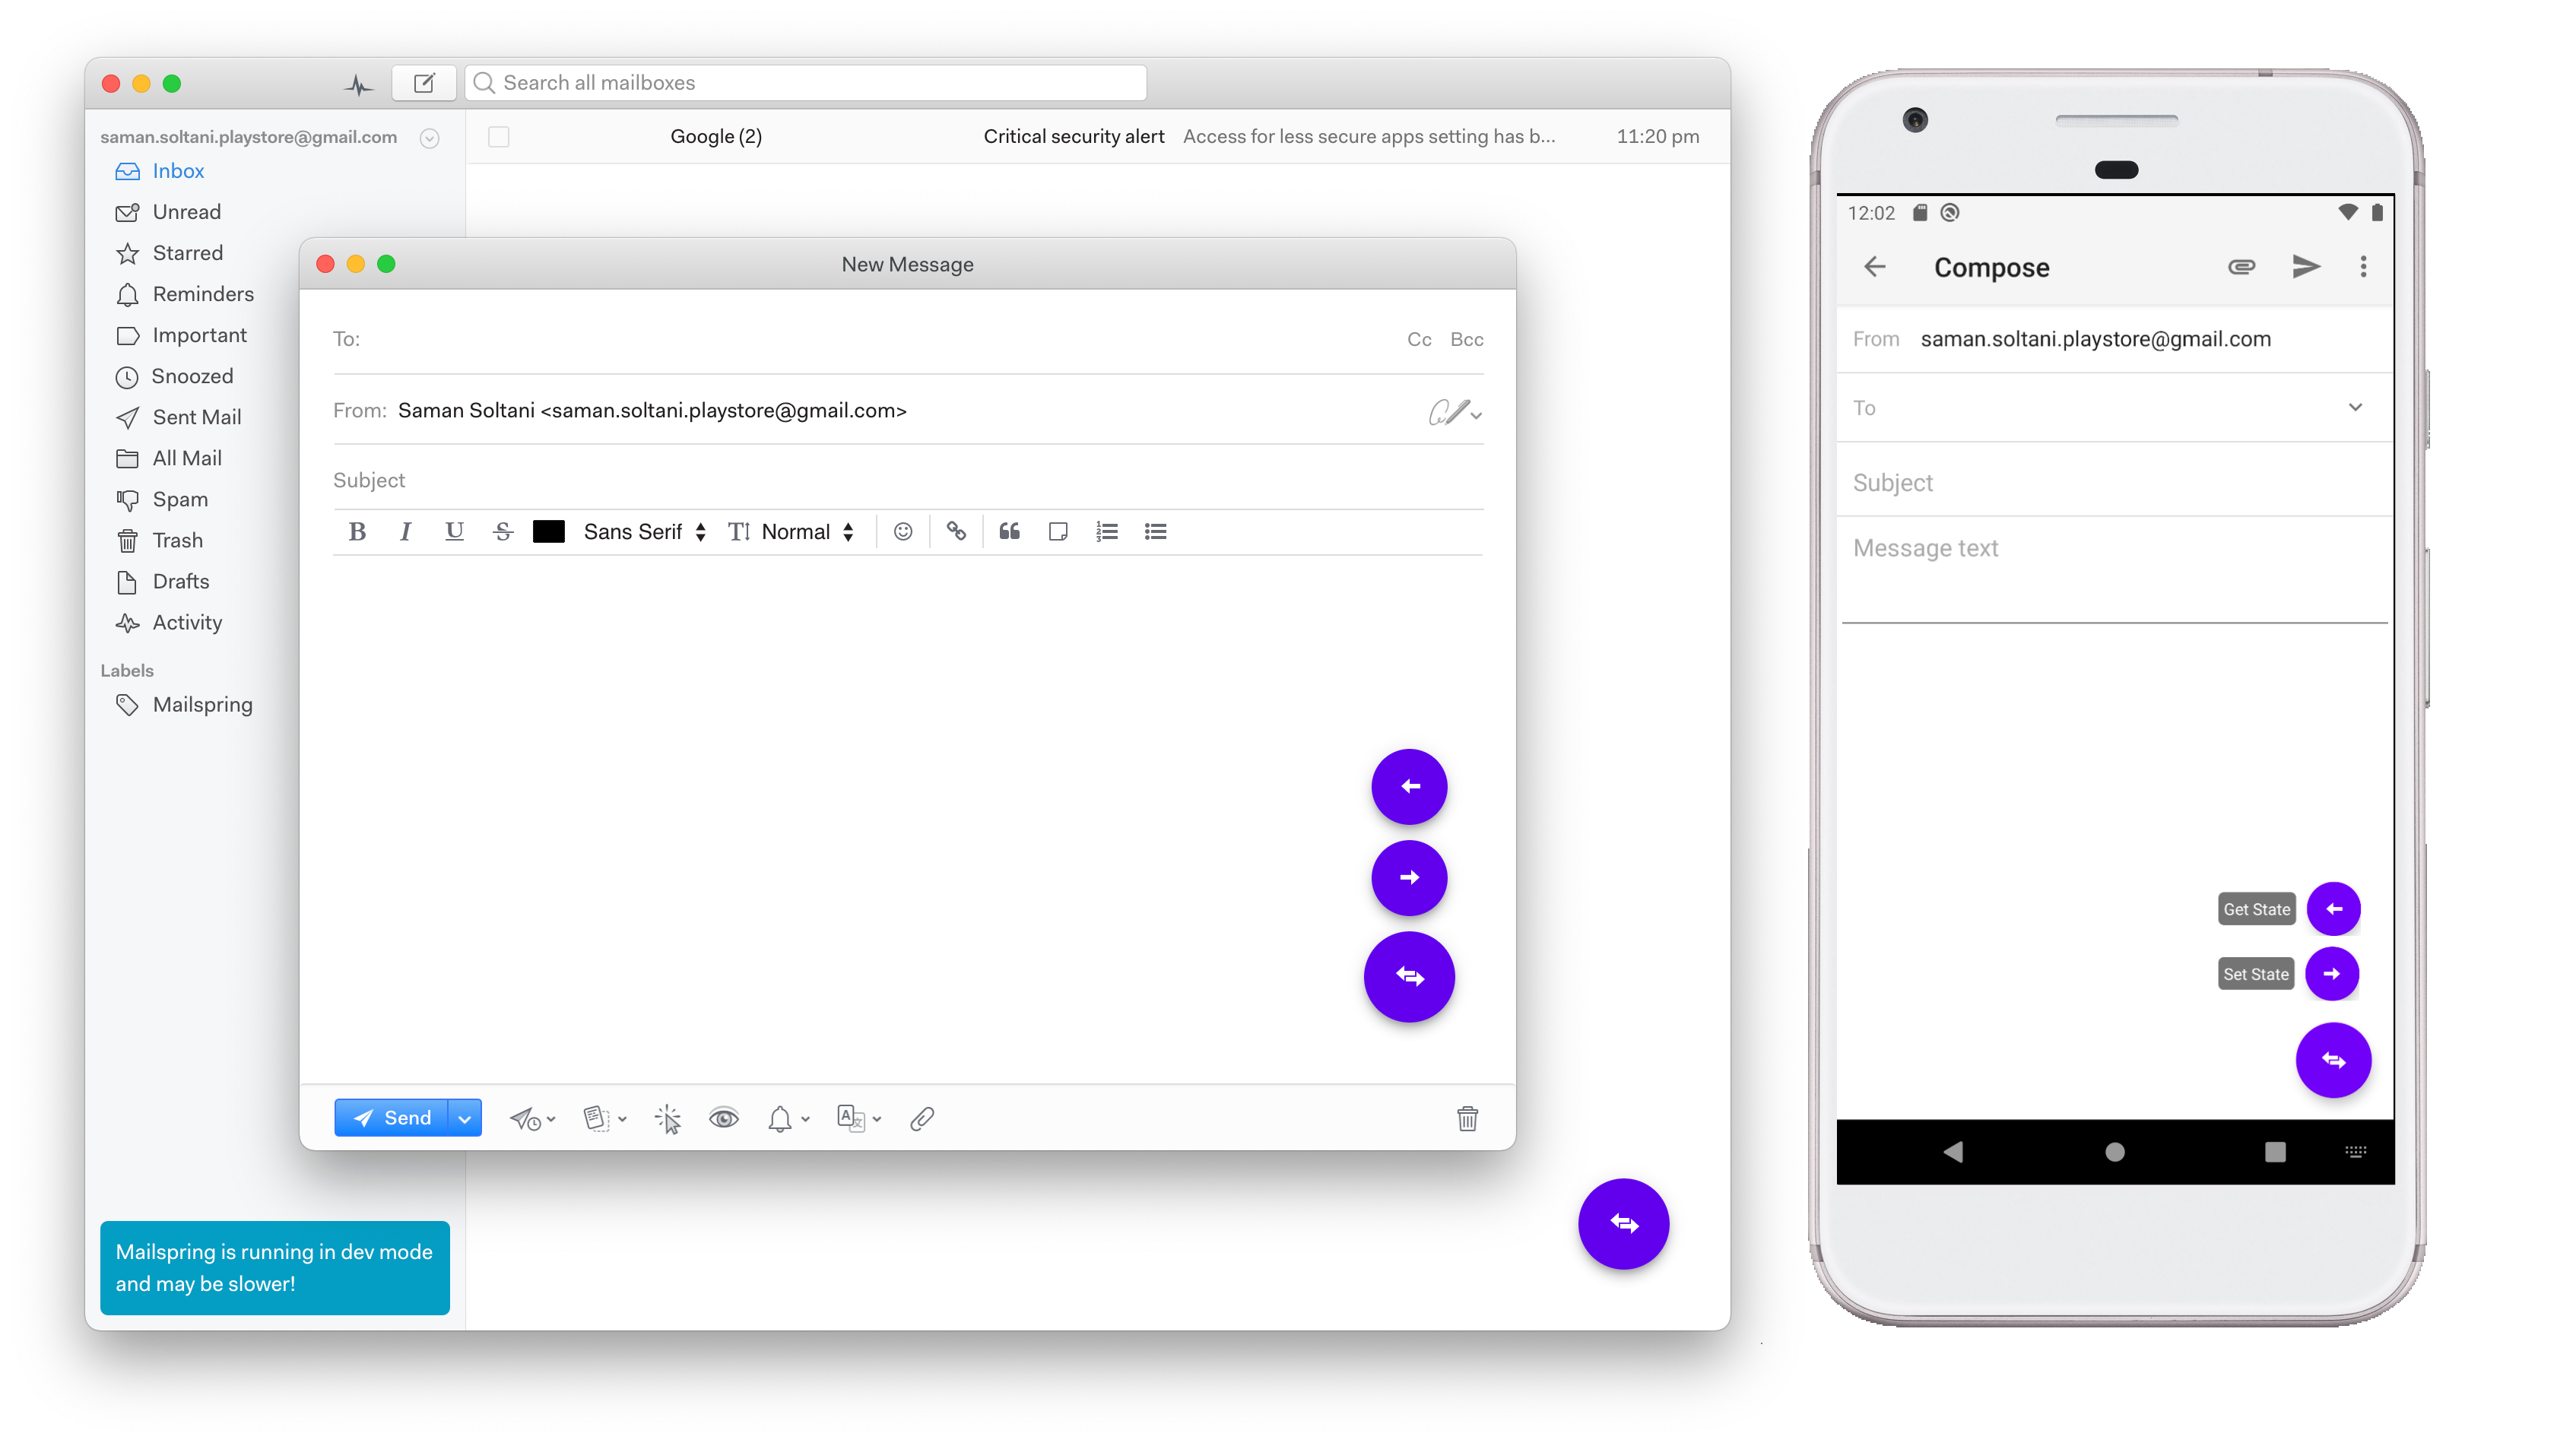
\includegraphics[width=\linewidth]{../figures/adapt-compose.png}
    \centering
    \caption{Screenshot of Compose Window}
    \label{fig:adapt-compose}
\end{figure}
\FloatBarrier

Figure \ref{fig:adapt-modal} shows the device modal of Mailspring and K-9 Mail which they have a migrate button.

\FloatBarrier
\begin{figure}[H]
    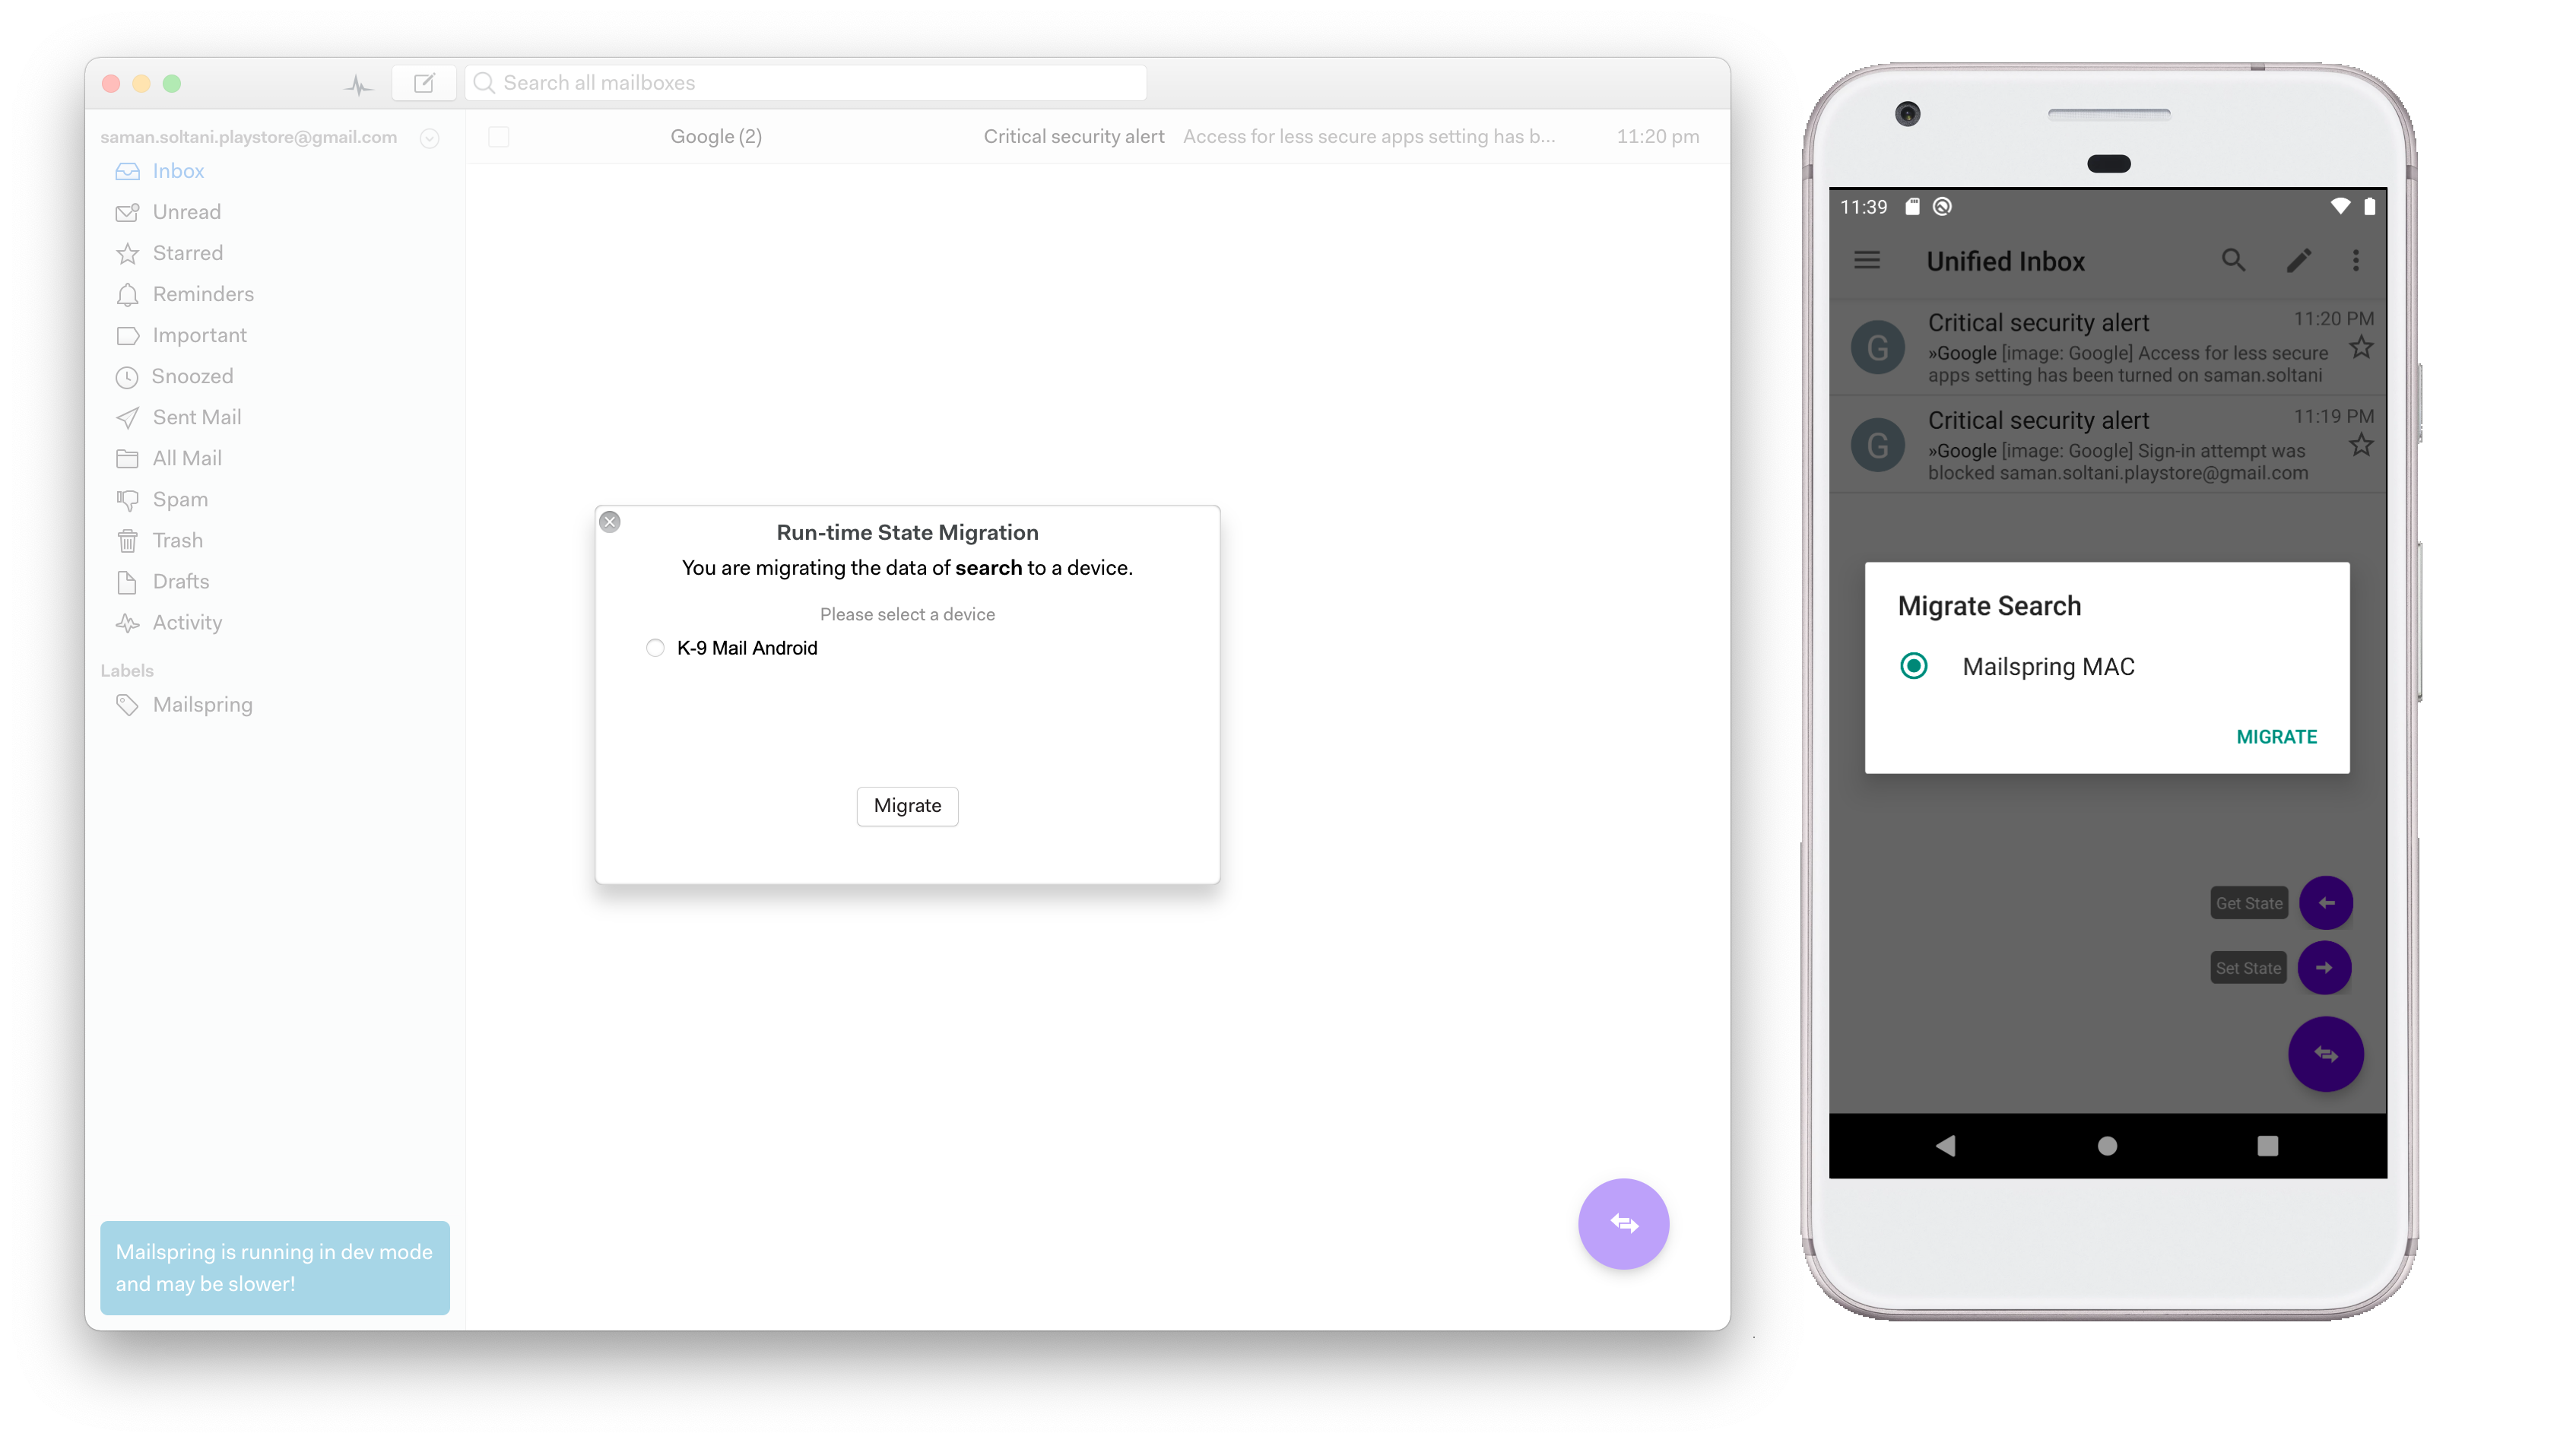
\includegraphics[width=\linewidth]{../figures/adapt-modal.png}
    \centering
    \caption{Screenshot of Device List Modal}
    \label{fig:adapt-modal}
\end{figure}
\FloatBarrier


